\section{Introduction}

\subsection{Motivation}


\begin{frame}{The Rise of online CoPs}
  \begin{itemize}
    \item World Wide Web is a place to meet and exchange information easily
    \item Researches transformed Communities of Practice into online Communities of Practice (CoPs)
          \begin{itemize}
            \item World-wide collaboration
            \item Fast information exchange
            \item Community Information Systems (CIS) help structuring their work
          \end{itemize}
          %researchers in particular from all over the world can collaborate more easily 
          %what Cops are will be discussed in more detail later.
    \item A CoP is only sustainable, if members continuously provide innovation efforts \cite{RKJa15}
    \item Therefore members need to be aware of their successes and failures to 
    \begin{itemize}
        \item predict future challenges and opportunities
        \item ensure the survival of the CoP
    \end{itemize}
  \end{itemize}

\end{frame}

\begin{frame}{Measuring Success}
  \begin{itemize}
    \item Success of CoP relies on success factors
    \item It is difficult to measure and evaluate those factors
          \begin{itemize}
            \item Factors are changing over time \cite{Renz16}
            \item Domain-specific success factors
          \end{itemize}
    \item Time consuming
    \item Traditional success modeling systems automate success evaluation
          \begin{itemize}
            \item Complicated interfaces
            \item Not optimized for collaboration
            \item Do not take mobility into consideration \cite{Renz16}
          \end{itemize}
  \end{itemize}
\end{frame}

\begin{frame}{Chat platforms}
  %this is why some continuous success modeling systems have been developed
  %however, the problem is that
  Social Networks and chat platforms are used for information exchange
  \begin{itemize}
    \item Familiar to most users
    \item Intuitive to use
    \item Real-time collaboration
    \item Optimized for mobile devices
  \end{itemize}
  %This shows how chat platforms could address the aforementioned issues
\end{frame}


\subsection{Thesis Goals}

\begin{frame}{Thesis Goals}
  \begin{itemize}
    \item Design a chatbot for success modeling and visualizations for a CIS
    \begin{itemize}
        \item Simplify the success modeling process
    \end{itemize}
        %   \begin{itemize}
        %     \item Bot should communicate with MobSOS (CCA) %framework
        %     \item Should be deployed with the Social Bot Framework
        %   \end{itemize}
    \item Find out how the bot affects collaboration and success awareness of the community %in contrast to traditional web frontends
  \end{itemize}
\end{frame}







\section{State of the Art}

\subsection{Social Bots}
\begin{frame}{Social Bots and Chatbots}
  \begin{block}{Definition}
    ``A social bot is a computer algorithm that automatically produces content and interacts with humans on social media, \dots'' \cite{FVD*16b}
  \end{block}
\end{frame}

\begin{frame}{Social Bots and Chatbots}
%   \begin{block}{Definition}
%     ``A social bot is a computer algorithm that automatically produces content and interacts with humans on social media, \dots'' \cite{FVD*16b}
%   \end{block}
  \begin{itemize}
    \item integrate automation into daily lives of users  %e.g. Alexa Smart Home, Shopping lists Reminders
    \item Users interact with bots by voice or chat %in the case of chat: Chatbots
    \item Provide better user experience, compared to traditional interfaces, as they are more intuitive to use
    \item Engage users in human-like conversations 
    \item Use Natural Language Understanding to determine users' intent
\end{itemize}
\end{frame}


\subsection{Success in Communities of Practice}
\begin{frame}{Communities of Practice}
  \begin{block}{Definition}
    ``Communities of practice are groups of people who share a concern or a
    passion for something they do and learn how to do it better as they interact regularly.'' \cite{Weng98}
  \end{block}
\end{frame}

\begin{frame}{Communities of Practice}
%   \begin{block}{Definition}
%     ``Communities of practice are groups of people who share a concern or a
%     passion for something they do and learn how to do it better as they interact regularly.'' \cite{Weng98}
%   \end{block}
  \begin{itemize}
    \item CoPs are diverse communities, which study a certain domain
    \item Learner is actively participating in the work of the community
    \begin{itemize}
        \item Naturally gains knowledge in the domain
    \end{itemize}
    \item CoPs make the learning process easier and faster \cite{CuZe05}
    \item Informal structures with permeable boundaries \cite{RKJa15}
          %informal structures: This means that there are no strict rules about the hierarchy inside a community and they do not follow the same structure as traditional organizations
          %Permeable boundaries: This means that it is not clearly defined which members belong to the CoP and which don't
    \item CoPs contain sub-communities which can be overlapping
          % members can belong to more than one community
  \end{itemize}
\end{frame}


% \begin{frame}{Members of a Communitiy of Practice}
%   \begin{itemize}
%     \item Have various roles
%           \begin{itemize}
%             \item Researchers
%             \item Professionals
%             \item Students
%             \item Hobbyists
%           \end{itemize} %DBIS and ACIS as an example????
%     \item Have different degrees of
%           \begin{itemize}
%             \item Knowledge %Researchers > students
%             \item Interest %Professionals > Hobbyists
%             \item Contribution
%                   \begin{itemize}
%                     \item Core Members %do most of the contribution 
%                     \item Lurkers %only consume but almost no contribution
%                           %study on open Source found that for random projects 22percent contribute. For the top 500 projects: ~90percent don't contribute -> 1% (90-9-1) rule
%                   \end{itemize}
%           \end{itemize}
%     \item Do not have to belong to the same organization
%     \item Share their work through social interaction e.g. online Social Networks %in this case we also talk about an online CoP
%   \end{itemize}
% \end{frame}


\begin{frame}{Measurement of Success}
  \begin{columns}
    \begin{column}[]{0.3\textwidth}
      \begin{itemize}
        \item Communities of Practice need to be aware of their success
              \begin{itemize}
                \item Improve their work
                \item Adjust to current trends
              \end{itemize}
              %Success seems to be a very abstract metric so in order to measure it we build a success model
              \item Measurement of Success of a Community Information System \textbf{CIS} through a \emph{Success Model}
              \item Success model \textbf{distinct} for each community
              %based on the goals that they want to achieve
              %e.g. a community of web developers: front end developers have different goals  than backend developers (beautiful animations vs informative (plain html))
      \end{itemize}
    \end{column}
    \begin{column}[]{0.7\textwidth}
      \begin{figure}
        \centering
        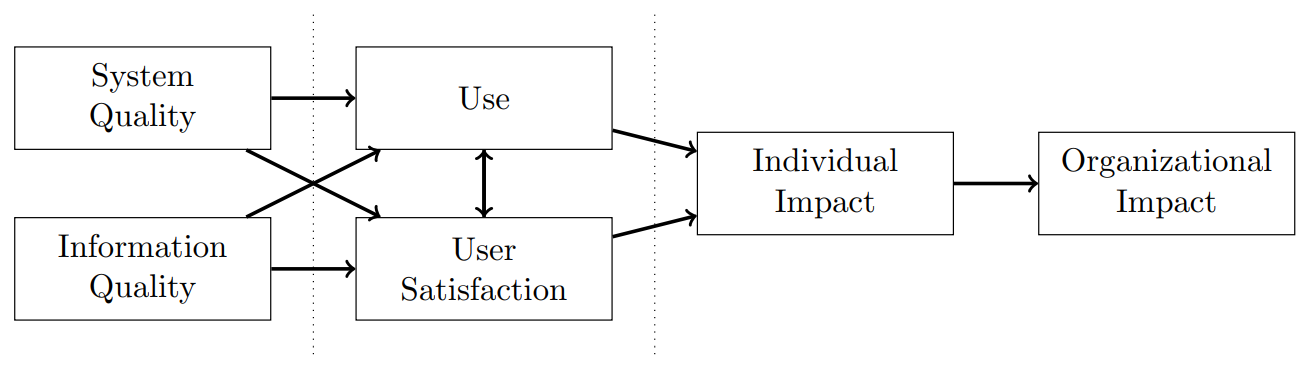
\includegraphics[width=\textwidth]{related_work/deloneMclean.png}
        \caption{CIS Success Model by DeLone and McLean \cite{DeMc92}}
        %13!!!!
      \end{figure}
    \end{column}
  \end{columns}
\end{frame}



\begin{frame}{MobSOS}

  \begin{itemize}
    \item MobSOS success model is based on the success model of DeLone and McLean
    \item Core Component of las2peer
    \item Monitors las2peer services
    \begin{itemize}
        \item MobSOS Success Modeling
        \item MobSOS Data Processing
    \end{itemize}
    \item MobSOS Continuous Community Analytics \cite{Kers20} extends MobSOS
          \begin{itemize}
            \item Provides visualizations of MobSOS data
            \item Ability to dynamically add databases
            \item GraphQL API
            \item REST API
          \end{itemize}
  \end{itemize}
  %The MobSOS cca also allows the addition of Mediabases, which can be used to gather data produced outside the las2peer environment
\end{frame}

% \begin{frame}{Mediabase}
%   \begin{columns}

%     \begin{column}[]{0.4\textwidth}
%       \begin{itemize}
%         \item Proposed to handle Web 2.0 data in a more effective way
%         \item Mediabase includes
%               \begin{itemize}
%                 \item Backend database (DB2 or MySQL)
%                 \item Crawler scripts
%                 \item Monitoring processes
%                 \item Frontend for user interactions
%               \end{itemize}
%       \end{itemize}
%     \end{column}

%     \begin{column}[]{0.6\textwidth}
%       \begin{figure}[h]
%         \centering
%         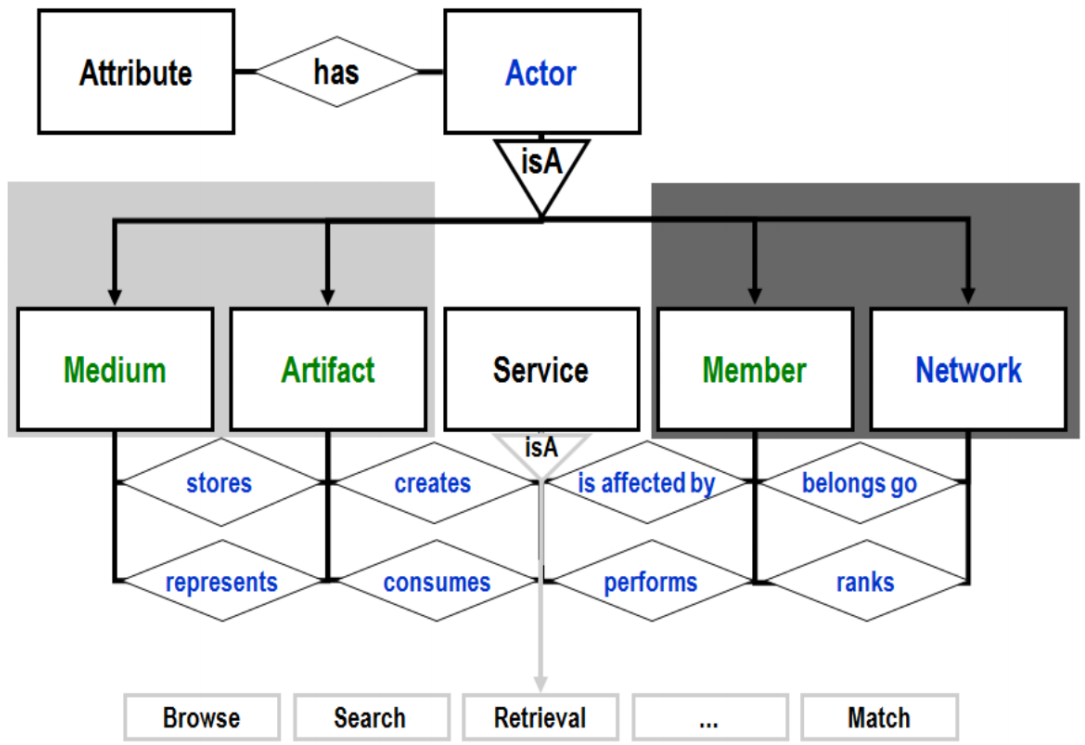
\includegraphics[height=0.8\textheight]{related_work/mediabase.png}
%         \caption{Mediabase Overview \cite{Klam10e}}
%       \end{figure}
%     \end{column}

%   \end{columns}
% \end{frame}



\section{Concept}
\subsection{Use Case}
\begin{frame}{Mensa Communities}
  \begin{itemize}
    \item Community of people frequently visiting the mensa
    \item Community consists of students and university employees
    \item Similar to the concept of Community of Practice %share a concern: food at the canteen. And Interact regularly: Students arguing on which mensa is the best?? Frequent visits to mensa
    % \item Different community levels:
    %       \begin{itemize}
    %         \item Top level: all mensa frequenters in Germany
    %         \item Intermediate level: all mensa frequenters for a University
    %         \item Low level: individual circle of friends, which frequent the canteen together %Members can belong to different circles of friends->overlapping
    %       \end{itemize}
  \end{itemize}
\end{frame}



\begin{frame}{mensabot}
  \begin{columns}
    \begin{column}[]{0.3\textwidth}
      For this community a chatbot called \emph{mensabot} is designed, which can be used to
  \begin{itemize}
    \item Get the menu for a canteen
    \item Rate meals
    \item Query success visualizations designed by the community
    \item Modify the success model of the community
  \end{itemize}
  The chatbot is deployed to Slack.
    \end{column}
    \begin{column}[]{0.7\textwidth}
      \begin{figure}
            \centering
            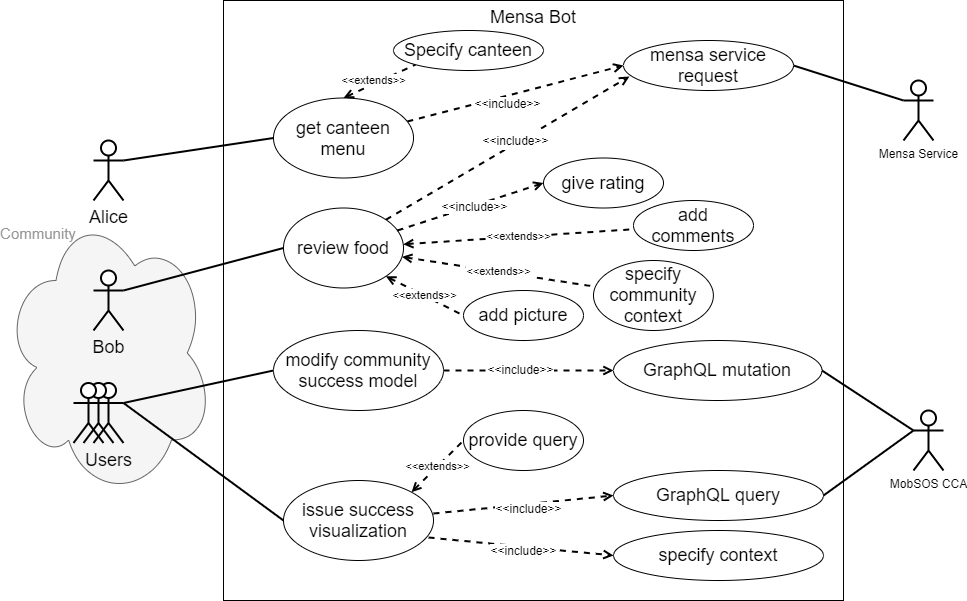
\includegraphics[height=0.85\textheight]{concept/usecase.png}
          \end{figure}
      \end{column}     
  \end{columns}
\end{frame}

% \begin{frame}{Use case diagram for the Chatbot}
%   \begin{figure}
%     \centering
%     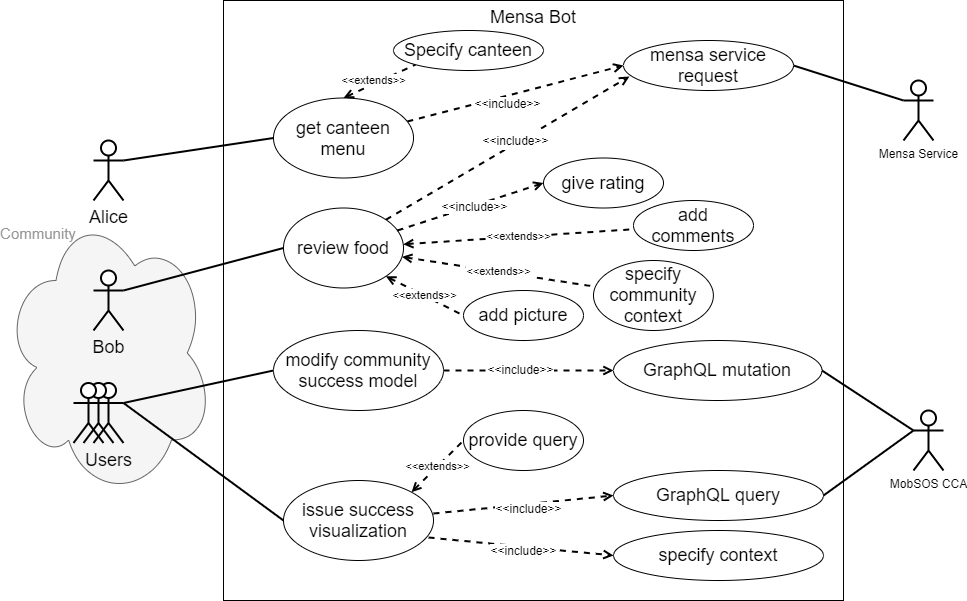
\includegraphics[height=0.85\textheight]{concept/usecase.png}
%   \end{figure}
% \end{frame}

% \subsection{System overview}

% \begin{frame}{System overview}
%   \begin{figure}
%     \centering
%     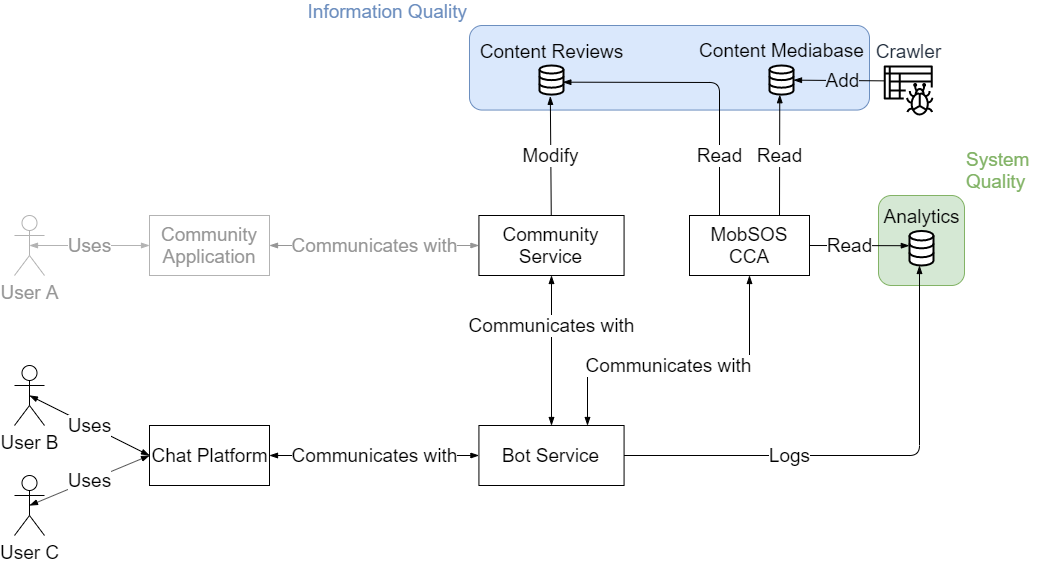
\includegraphics[height=0.85\textheight]{realization/Component_Diagramm.png}

%     \label{fig:sytsemOverview}
%   \end{figure}
% \end{frame}

\section{Realization}

\begin{frame}\begin{columns}
    \begin{column}[]{0.7\textwidth}
      \begin{figure}
        \centering
        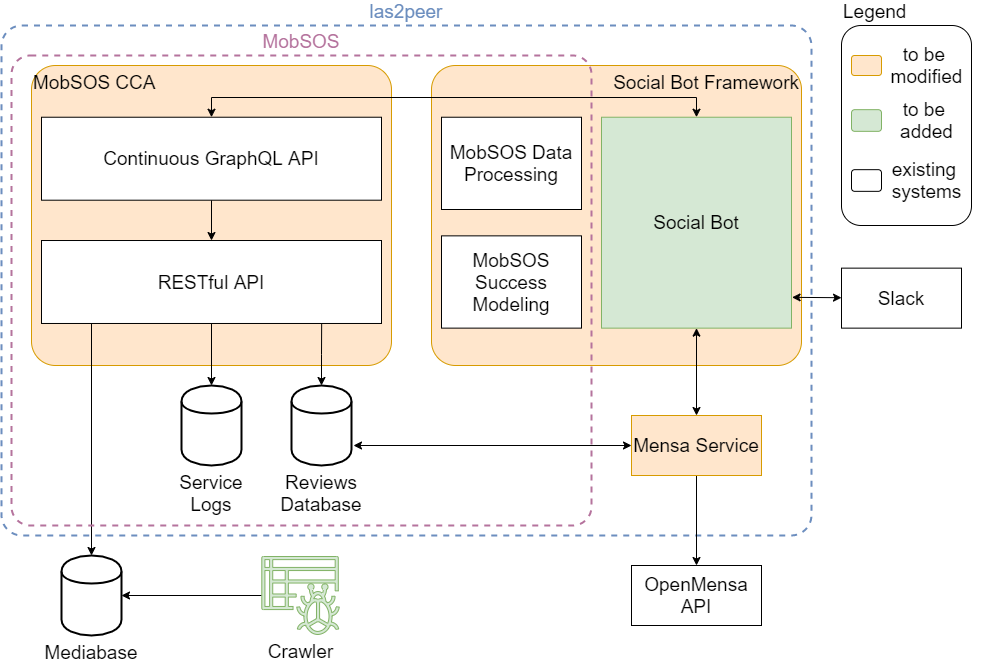
\includegraphics[height=0.9\textheight]{realization/components_overview.png}
        \caption{Overview of the different components}
        \label{fig:componentsOverview}
      \end{figure}
    \end{column}
    \begin{column}[]{0.3\textwidth}
      Technologies:
      \begin{itemize}
        \item Chat Platform (Slack)
        \item las2peer
        \item Social Bot Manager
        \item Mensa Service
        \item MobSOS
              \begin{itemize}
                \item MobSOS CCA GraphQL API
                \item MobSOS CCA REST API
                \item MobSOS Data Processing
                \item MobSOS Success Modeling
              \end{itemize}
        \item Mediabase
              \begin{itemize}
                \item JavaScript Crawler
              \end{itemize}
      \end{itemize}
    \end{column}
  \end{columns}
\end{frame}

\begin{frame}{Example of a visualization request}
    
    \begin{columns}
        \begin{column}[t]{0.5\textwidth}
            \begin{figure}
               
                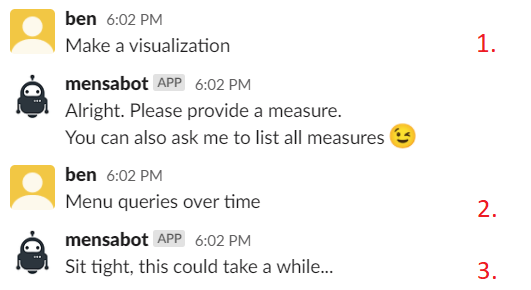
\includegraphics[width=\textwidth]{realization/bot/visual_alt1_anot.png} 
            \end{figure}
        \end{column}
        \begin{column}[t]{0.5\textwidth}
            \begin{enumerate}
              \item intent visualization is recognized
              \begin{itemize}
                \item Visualization routine is triggered
              \end{itemize}
              \item user message is passed to success modeling service
            \item success modeling service prepares the visualization
            \begin{itemize}
              \item extract the measure from the catalog
              \item CCA GraphQL request for data
              \item Data2Chart request to generate chart
              \item resulting chart is sent back to the bot manager
            \end{itemize}
            \end{enumerate}
        \end{column}
    \end{columns}
\end{frame}

\begin{frame}{Example of a visualization request}
  \begin{columns}
    \begin{column}[t]{0.5\textwidth}
      \begin{figure}
        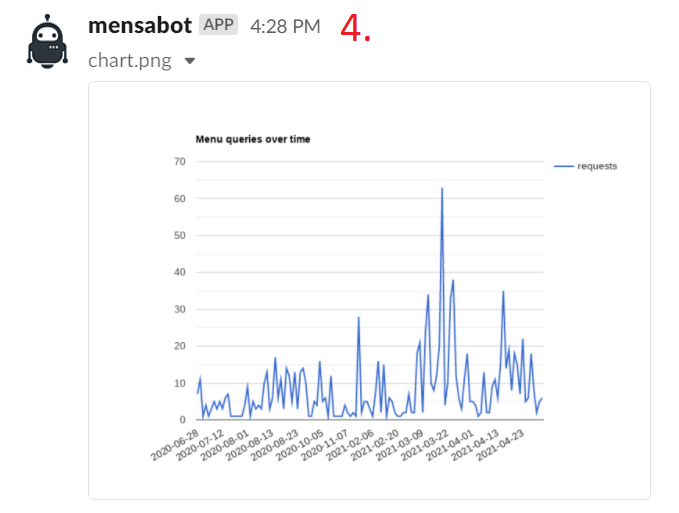
\includegraphics[width=.8\textwidth]{realization/bot/visual_alt2.png} 
      \end{figure}
    \end{column}
    \begin{column}[]{0.5\textwidth}
      \begin{enumerate}
        \setcounter{enumi}{3}
        \item mensabot displays the chart in the chat
      \end{enumerate}
    \end{column}
  \end{columns}
\end{frame}

\section{Evaluation}
\begin{frame}{Research Questions}
  \begin{enumerate}
    \item Does the use of chatbots increase the success awareness of the community?
    \item Does it increase collaboration between members?
    % \item Does it improve the user experience in terms of mobility?
  \end{enumerate}
\end{frame}


\begin{frame}{The requirements of the community}
  \begin{itemize}
    \item We conducted a survey to figure out the requirements of the community
    \item Participants were asked to rank success factors based on perceived relevance
    \item Success model contains the most popular success factors
  \end{itemize}
\end{frame}

\begin{frame}{Evaluation of canteen specific task}
  \begin{columns}
    \begin{column}[t]{0.5\textwidth}
      \begin{figure}[H] 
   \centering
    \begin{tikzpicture}
      \begin{axis}
        [xmin=0.9,xmax=5.1,
            label style={font=\footnotesize},
            tick label style={font=\footnotesize},
            yticklabels,
            height=4.5cm,width=8cm,ytick={1,2,3,4,5,6,7},ylabel={Average User Rating }
           ,scatter/classes={
          a={mark=,red!50!black},
          b={mark=,blue!50!black},
          c={mark=,green!50!black},
          d={mark=,white!50!black}
         },title={"I could imagine myself using this bot to get the menu."}]
        
        \addplot[color=blue,
        boxplot prepared={
          median= 4,
          upper quartile=5,
          lower quartile=3,
          upper whisker=5,
          lower whisker=1,
        },
         ] coordinates {}; 
    
         \addplot[scatter,only marks,scatter src=explicit symbolic] 
       table [
         y=y,
         x=x
        ]
    {
    x y 
    4 1 
    
    };
    \node[align=center, text=black]
    at (axis cs:4,1.2) {\scalebox{0.8}{SD=1.5}};
      \end{axis}
    \end{tikzpicture}
   

    \begin{tikzpicture}
        \begin{axis}
            [xmin=0.9,xmax=5.1,
            label style={font=\footnotesize},
            tick label style={font=\footnotesize},
            yticklabels,
            height=4.5cm,width=8cm,ytick={1,2,3,4,5,6,7},ylabel={Average User Rating}
           ,scatter/classes={
          a={mark=,red!50!black},
          b={mark=,blue!50!black},
          c={mark=,green!50!black},
          d={mark=,white!50!black}
         },title={"I could imagine myself using the bot to make reviews."}]
          \addplot[color=blue,
          boxplot prepared={
            median=4,
            upper quartile=5,
            lower quartile=3,
            upper whisker=5,
            lower whisker=1,
          },
           ] coordinates {}; 
      
           \addplot[scatter,only marks,scatter src=explicit symbolic] 
         table [
           y=y,
           x=x
          ]
      {
      x y 
      4 1 
      };
      \node[align=center, text=black]
      at (axis cs:4,1.2) {\scalebox{0.8}{SD=1.27}};
        \end{axis}
      \end{tikzpicture}
      \caption{Usability of the bot to get the menu and write reviews}
      \label{fig:canteenPlot1}
      \end{figure}
    \end{column}
    \begin{column}[t]{0.5\textwidth}
      \begin{figure}[H] 
    \centering
    \begin{tikzpicture}
      \begin{axis}
          [xmin=0.9,xmax=5.1,
          label style={font=\footnotesize},
          tick label style={font=\footnotesize},
          yticklabels,
          height=4.5cm,width=8cm,ytick={1,2,3,4,5,6,7},ylabel={Average User Rating }
         ,scatter/classes={
        a={mark=,red!50!black},
        b={mark=,blue!50!black},
        c={mark=,green!50!black},
        d={mark=,white!50!black}
       },title={"Making reviews is useful for the community."}]
        \addplot[color=blue,
        boxplot prepared={
          median= 5,
          upper quartile=5,
          lower quartile=4,
          upper whisker=5,
          lower whisker=3,
        },
         ] coordinates {}; 
    
         \addplot[scatter,only marks,scatter src=explicit symbolic] 
       table [
         y=y,
         x=x
        ]
    {
    x y 
    4.58 1 
    };
    \node[align=center, text=black]
    at (axis cs:4.5,1.2) {\scalebox{0.8}{SD=0.69}};
      \end{axis}
    \end{tikzpicture}

  \caption{Importance of reviews to the community}
  \label{fig:canteenPlot2}
  \end{figure}
    \end{column}
  \end{columns}
\end{frame}

\begin{frame}{Evaluation of visualization task}
  \begin{columns}
    \begin{column}[t]{0.5\textwidth}
      % \begin{figure}[H] 
%     \centering
%     \begin{tikzpicture}
%       \begin{axis}
%         [xmin=0.9,xmax=5.1,
%             label style={font=\footnotesize},
%             tick label style={font=\footnotesize},
%             yticklabels,
%             height=4.5cm,width=8cm,ytick={1,2,3,4,5,6,7},ylabel={Average User Rating }
%            ,scatter/classes={
%           a={mark=,red!50!black},
%           b={mark=,blue!50!black},
%           c={mark=,green!50!black},
%           d={mark=,white!50!black}
%          },title={"I understood the visualizations without needing explanations."}]
         
       
%         \addplot[color=blue,
%         boxplot prepared={
%           median= 5,
%           upper quartile=5,
%           lower quartile=4,
%           upper whisker=5,
%           lower whisker=2,
%         },
%          ] coordinates {}; 
    
%          \addplot[scatter,only marks,scatter src=explicit symbolic] 
%        table [
%          y=y,
%          x=x
%         ]
%     {
%     x y 
%     4.37 1 
    
%     };
%     \node[align=center, text=black]
%     at (axis cs:4.5,1.2) {\scalebox{0.8}{SD=0.9}};
%       \end{axis}
%     \end{tikzpicture}
    
%     \begin{tikzpicture}
%         \begin{axis}
%             [xmin=0.9,xmax=5.1,
%             label style={font=\footnotesize},
%             tick label style={font=\footnotesize},
%             yticklabels,
%             height=4.5cm,width=8cm,ytick={1,2,3,4,5,6,7},ylabel={Average User Rating }
%            ,scatter/classes={
%           a={mark=,red!50!black},
%           b={mark=,blue!50!black},
%           c={mark=,green!50!black},
%           d={mark=,white!50!black}
%          },title={"The size inside the visualizations was large enough to be read inside the chat."}]
          
%           \addplot[color=blue,
%           boxplot prepared={
%             median= 4,
%             upper quartile=5,
%             lower quartile=4,
%             upper whisker=5,
%             lower whisker=1,
%           },
%            ] coordinates {}; 
      
%            \addplot[scatter,only marks,scatter src=explicit symbolic] 
%          table [
%            y=y,
%            x=x
%           ]
%       {
%       x y 
%       4.11 1 
%       };
%       \node[align=center, text=black]
%       at (axis cs:4.5,1.2) {\scalebox{0.8}{SD=1.1}};
%         \end{axis}
%     \end{tikzpicture}
% \end{figure}
\begin{figure}[] 
  \begin{tikzpicture}
    \begin{axis}
      [xmin=0.9,xmax=5.1,
      height=11cm,width=10cm,ytick={1,2,3,4,5,6,7,8,9,10},
                      label style={font=\footnotesize},
                      tick label style={font=\footnotesize}, yticklabel style={align=right},ylabel={Average User Rating (N=20)},
      yticklabels={I understood the visualizations \\without needing explanations.,The size inside the visualizations \\was large enough to \\be read inside the chat. },scatter/classes={
    a={mark=*,red!50!black},
    b={mark=*,blue!50!black},
    c={mark=*,green!50!black},
    d={mark=*,white!50!black}
   }]
   \addplot[color=blue,
    boxplot prepared={
      median= 4,
      upper quartile=5,
      lower quartile=4,
      upper whisker=5,
      lower whisker=2,
    },
      ] coordinates {}; 
      \addplot[color=blue,
      boxplot prepared={
        median= 4,
        upper quartile=5,
        lower quartile=4,
        upper whisker=5,
        lower whisker=1,
      },
        ] coordinates {};  
    
       \addplot[scatter,only marks,scatter src=explicit symbolic] 
          table [
              y=y,
              x=x
              ]
          {
          x y 
          4.37 1
          4.11 2  
          };
          \node[align=center, text=black]
          at (axis cs:4.5,2.2) {\scalebox{0.8}{SD=1.1}};
          \node[align=center, text=black]
          at (axis cs:4.5,1.2) {\scalebox{0.8}{SD=0.9}};
    \end{axis}
  \end{tikzpicture}
  
\end{figure}
    \end{column}
    \begin{column}[t]{0.5\textwidth}
      
% \begin{figure}[h]
%   \centering
%   \begin{tikzpicture}
%       \begin{axis}
%           [xmin=0.9,xmax=5.1,
%           label style={font=\footnotesize},
%           tick label style={font=\footnotesize},
%           yticklabels,
%           height=4.5cm,width=8cm,ytick={1,2,3,4,5,6,7},ylabel={Average User Rating }
%          ,scatter/classes={
%         a={mark=,red!50!black},
%         b={mark=,blue!50!black},
%         c={mark=,green!50!black},
%         d={mark=,white!50!black}
%        },title={"I could imagine myself using this bot to make visualizations."}]
       
%         \addplot[color=blue,
%         boxplot prepared={
%           median= 4,
%           upper quartile=5,
%           lower quartile=3,
%           upper whisker=5,
%           lower whisker=1,
%         },
%          ] coordinates {}; 
    
%          \addplot[scatter,only marks,scatter src=explicit symbolic] 
%        table [
%          y=y,
%          x=x
%         ]
%     {
%     x y 
%     3.95 1 
%     };
%     \node[align=center, text=black]
%     at (axis cs:4,1.2) {\scalebox{0.8}{SD=1.18}};
%       \end{axis}
%     \end{tikzpicture}
% \end{figure}

% \begin{figure}
%     \centering
    
%     \begin{tikzpicture}
%         \begin{axis}
%             [xmin=0.9,xmax=5.1,
%             label style={font=\footnotesize},
%             tick label style={font=\footnotesize},
%             yticklabels,
%             height=4.5cm,width=8cm,ytick={1,2,3,4,5,6,7},ylabel={Average User Rating }
%            ,scatter/classes={
%           a={mark=,red!50!black},
%           b={mark=,blue!50!black},
%           c={mark=,green!50!black},
%           d={mark=,white!50!black}
%          },title={"Using the chatbot for visualizations increases the success awareness in the community."}]
%           \addplot[color=blue,
%           boxplot prepared={
%             median= 4,
%             upper quartile=5,
%             lower quartile=3,
%             upper whisker=5,
%             lower whisker=1,
%           },
%            ] coordinates {}; 
      
%            \addplot[scatter,only marks,scatter src=explicit symbolic] 
%          table [
%            y=y,
%            x=x
%           ]
%       {
%       x y 
%       4 1 
%       };
%       \node[align=center, text=black]
%       at (axis cs:4,1.2) {\scalebox{0.8}{SD=1.15}};
%         \end{axis}
%     \end{tikzpicture}
    
% \end{figure}

\begin{figure}[] 
  \begin{tikzpicture}
    \begin{axis}
      [xmin=0.9,xmax=5.1,
      height=11cm,width=10cm,ytick={1,2,3,4,5,6,7,8,9,10},
                      label style={font=\footnotesize},
                      tick label style={font=\footnotesize}, yticklabel style={align=right},ylabel={},
      yticklabels={Using the chatbot for visualizations \\increases the success awareness \\in the community.,I could imagine myself using this bot \\to make visualizations. },scatter/classes={
    a={mark=*,red!50!black},
    b={mark=*,blue!50!black},
    c={mark=*,green!50!black},
    d={mark=*,white!50!black}
   }]
   \addplot[color=blue,
    boxplot prepared={
      median= 4,
      upper quartile=5,
      lower quartile=3,
      upper whisker=5,
      lower whisker=1,
    },
    ] coordinates {}; 
    \addplot[color=blue,
    boxplot prepared={
      median= 4,
      upper quartile=5,
      lower quartile=3,
      upper whisker=5,
      lower whisker=1,
    },
      ] coordinates {}; 
    
       \addplot[scatter,only marks,scatter src=explicit symbolic] 
          table [
              y=y,
              x=x
              ]
          {
          x y 
          4 2
          3.95 1  
          };
          \node[align=center, text=black]
           at (axis cs:4,2.2) {\scalebox{0.8}{SD=1.18}};
          \node[align=center, text=black]
          at (axis cs:3.95,1.2) {\scalebox{0.8}{SD=1.15}};
    \end{axis}
  \end{tikzpicture}
  
\end{figure}
    \end{column}
  \end{columns}
\end{frame}


\begin{frame}{Evaluation of success modeling task}
 
      
\begin{figure}[H] 
    \centering
    \begin{tikzpicture}
      \begin{axis}
        [xmin=0.9,xmax=5.1,
        label style={font=\footnotesize},
        tick label style={font=\footnotesize},
        yticklabels,
        height=4.5cm,width=8cm,ytick={1,2,3,4,5,6,7},ylabel={Average User Rating }
       ,scatter/classes={
      a={mark=,red!50!black},
      b={mark=,blue!50!black},
      c={mark=,green!50!black},
      d={mark=,white!50!black}
     },title={"I could imagine using the bot to add measures to the success model"}]
        \addplot[color=blue,
        boxplot prepared={
          median= 5,
          upper quartile=5,
          lower quartile=4,
          upper whisker=5,
          lower whisker=2,
        },
         ] coordinates {}; 
    
         \addplot[scatter,only marks,scatter src=explicit symbolic] 
       table [
         y=y,
         x=x
        ]
    {
    x y 
    4.5 1 
    
    };
    \node[align=center, text=black]
    at (axis cs:4.5,1.2) {\scalebox{0.8}{SD=1.38}};
      \end{axis}
    \end{tikzpicture}
\caption{}
\label{fig:SuccPlot1}
    
   
    
\end{figure}

   
      % 
\begin{figure}[H] 
    \centering
    \begin{tikzpicture}
        \begin{axis}
          [xmin=0.9,xmax=5.1,label style={font=\footnotesize},
            tick label style={font=\footnotesize},
          height=4.5cm,width=8cm,ytick={1,2,3,4,5,6,7}, ylabel={Average User Rating}, yticklabels,
         title={"Being able to edit the success model increases the success awareness of the community"},scatter/classes={
        a={mark=,red!50!black},
        b={mark=,blue!50!black},
        c={mark=,green!50!black},
        d={mark=,white!50!black}
       }]
          \addplot[color=blue,
          boxplot prepared={
            median= 4,
            upper quartile=5,
            lower quartile=3,
            upper whisker=5,
            lower whisker=1,
          },
           ] coordinates {}; 
      
           \addplot[scatter,only marks,scatter src=explicit symbolic] 
         table [
           y=y,
           x=x
          ]
      {
      x y 
      4 1 
      };
      \node[align=center, text=black]
      at (axis cs:4,1.2) {\scalebox{0.8}{SD=1.17}};
        \end{axis}
    \end{tikzpicture}
    \caption{}
    \label{fig:SuccPlot2}
   
    
\end{figure}

   
\end{frame}


% \begin{frame}{Overview}
%   \begin{itemize}
%     \item Find mensa community
%     \item Participants are part of the mensa community
%     \item Evaluation will be done on two phases:
%           \begin{itemize}
%             \item  Community Service Phase
%             \item Success Modeling Phase
%           \end{itemize}
%   \end{itemize}
% \end{frame}


% \begin{frame}{Community Service Phase}
%   \begin{itemize}
%     \item Evaluate the usability of the bot for getting menu and making reviews
%     \item Volunteers will join a new Mensa Slack group
%     \item The chatbot is included in a group channel
%           \begin{itemize}
%             \item can be used to query menu
%           \end{itemize}
%     \item Members are asked to make a food review by private chat with the bot
%     \item Hand out questionnaire covering usability of the bot
%     \item Feedback is included into the success model of the community
%   \end{itemize}
% \end{frame}

% \begin{frame}{Success Modeling Phase}
%   \begin{itemize}
%     \item Evaluate the collaboration aspect of the bot
%     \item Preferably same volunteers as first phase %maybe some new features were added in the first phase which they can now try out... See their impact on the community
%     \item Divide into groups of 2-3 students
%           \begin{itemize}
%             \item make visualization requests
%             \item update the success model
%           \end{itemize}
%           Use MobSOS CCA frontend and new chatbot
%     \item Hand out questionnaire covering collaboration and success awareness
%   \end{itemize}
% \end{frame}

% \section{Project Plan}
% \begin{frame}
%   \begin{figure}
%     \centering
%     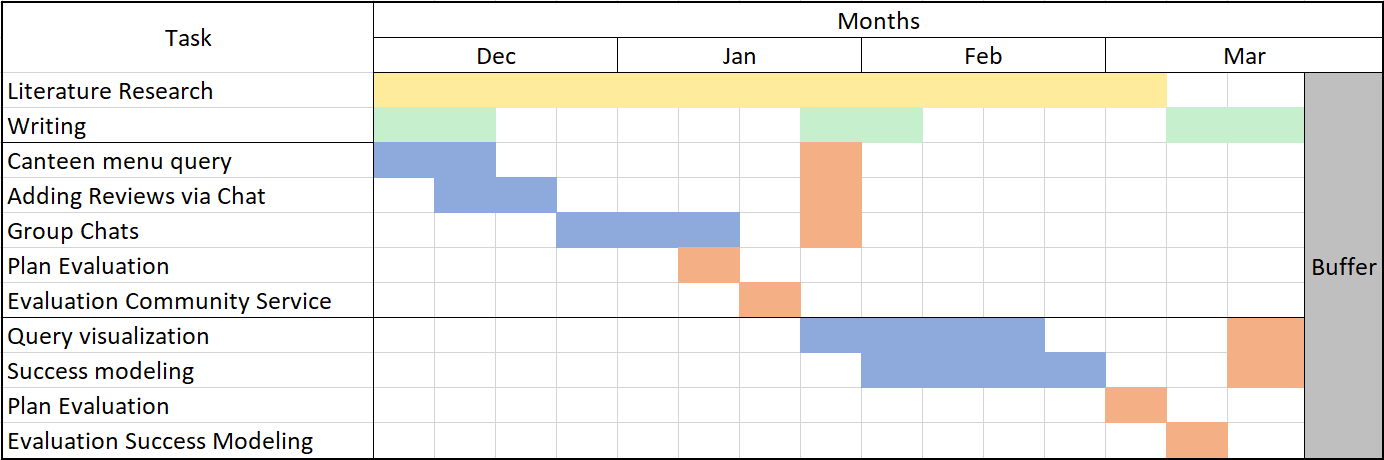
\includegraphics[width=0.89\textwidth]{project_plan/projectplan.png}
%     %bot can be used from first evaluation onwards
%   \end{figure}
% \end{frame}


% \section{First Section} % Sections can be created in order to organize your presentation into discrete blocks, all sections and subsections are automatically printed in the table of contents as an overview of the talk
% %------------------------------------------------

% \subsection{Subsection Example} % A subsection can be created just before a set of slides with a common theme to further break down your presentation into chunks

% \begin{frame}
% \frametitle{Paragraphs of Text}
% Sed iaculis dapibus gravida. Morbi sed tortor erat, nec interdum arcu. Sed id lorem lectus. Quisque viverra augue id sem ornare non aliquam nibh tristique. Aenean in ligula nisl. Nulla sed tellus ipsum. Donec vestibulum ligula non lorem vulputate fermentum accumsan neque mollis.\\~\\

% Sed diam enim, sagittis nec condimentum sit amet, ullamcorper sit amet libero. Aliquam vel dui orci, a porta odio. Nullam id suscipit ipsum. Aenean lobortis commodo sem, ut commodo leo gravida vitae. Pellentesque vehicula ante iaculis arcu pretium rutrum eget sit amet purus. Integer ornare nulla quis neque ultrices lobortis. Vestibulum ultrices tincidunt libero, quis commodo erat ullamcorper id.
% \end{frame}

% %------------------------------------------------

% \begin{frame}
% \frametitle{Bullet Points}
% \begin{itemize}
% \item Lorem ipsum dolor sit amet, consectetur adipiscing elit
% \item Aliquam blandit faucibus nisi, sit amet dapibus enim tempus eu
% \item Nulla commodo, erat quis gravida posuere, elit lacus lobortis est, quis porttitor odio mauris at libero
% \item Nam cursus est eget velit posuere pellentesque
% \item Vestibulum faucibus velit a augue condimentum quis convallis nulla gravida
% \end{itemize}
% \end{frame}

% %------------------------------------------------

% \begin{frame}
% \frametitle{Blocks of Highlighted Text}
% \begin{block}{Block 1}
% Lorem ipsum dolor sit amet, consectetur adipiscing elit. Integer lectus nisl, ultricies in feugiat rutrum, porttitor sit amet augue. Aliquam ut tortor mauris. Sed volutpat ante purus, quis accumsan dolor.
% \end{block}

% \begin{block}{Block 2}
% Pellentesque sed tellus purus. Class aptent taciti sociosqu ad litora torquent per conubia nostra, per inceptos himenaeos. Vestibulum quis magna at risus dictum tempor eu vitae velit.
% \end{block}

% \begin{block}{Block 3}
% Suspendisse tincidunt sagittis gravida. Curabitur condimentum, enim sed venenatis rutrum, ipsum neque consectetur orci, sed blandit justo nisi ac lacus.
% \end{block}
% \end{frame}

% %------------------------------------------------

% \begin{frame}
% \frametitle{Multiple Columns}
% \begin{columns}[c] % The "c" option specifies centered vertical alignment while the "t" option is used for top vertical alignment

% \column{.45\textwidth} % Left column and width
% \textbf{Heading}
% \begin{enumerate}
% \item Statement
% \item Explanation
% \item Example
% \end{enumerate}

% \column{.5\textwidth} % Right column and width
% Lorem ipsum dolor sit amet, consectetur adipiscing elit. Integer lectus nisl, ultricies in feugiat rutrum, porttitor sit amet augue. Aliquam ut tortor mauris. Sed volutpat ante purus, quis accumsan dolor.

% \end{columns}
% \end{frame}

% %------------------------------------------------
% \section{Second Section}
% %------------------------------------------------

% \begin{frame}
% \frametitle{Table}
% \begin{table}
% \begin{tabular}{l l l}
% \toprule
% \textbf{Treatments} & \textbf{Response 1} & \textbf{Response 2}\\
% \midrule
% Treatment 1 & 0.0003262 & 0.562 \\
% Treatment 2 & 0.0015681 & 0.910 \\
% Treatment 3 & 0.0009271 & 0.296 \\
% \bottomrule
% \end{tabular}
% \caption{Table caption}
% \end{table}
% \end{frame}

% %------------------------------------------------

% \begin{frame}
% \frametitle{Theorem}
% \begin{theorem}[Mass--energy equivalence]
% $E = mc^2$
% \end{theorem}
% \end{frame}

% %------------------------------------------------

% \begin{frame}[fragile] % Need to use the fragile option when verbatim is used in the slide
% \frametitle{Verbatim}
% \begin{example}[Theorem Slide Code]
% \begin{verbatim}
% \begin{frame}
% \frametitle{Theorem}
% \begin{theorem}[Mass--energy equivalence]
% $E = mc^2$
% \end{theorem}
% \end{frame}\end{verbatim}
% \end{example}
% \end{frame}

% %------------------------------------------------

% \begin{frame}
% \frametitle{Figure}
% Code to include your own image as figure~\ref{fig:acis} from the `Figure' directory.
% \begin{figure}
% 
\includegraphics[width=0.5\linewidth]{acis}
% \caption{Acis logo}
% \label{fig:acis}
% \end{figure}
% \end{frame}

% %------------------------------------------------

% \begin{frame}[fragile] % Need to use the fragile option when verbatim is used in the slide
% \frametitle{Citation}
% An example of the \verb|\cite| command to cite within the presentation:\\~

% This statement requires citation \cite{Weng98}.
% \end{frame}